\documentclass[dvipdfmx]{classes/tyukan}
\usepackage[final]{graphicx}

\Year{令和6}

\No{06}
\Name{糸川 倫太朗}
\Laboratory{青山研究室}

\Theme{A JavaScript compiler and TypeScript checker with a focus on
static analysis and runtime performance}
\Keywords{JavaScript, TypeScript, compiler, static analysis}

\begin{document}

\paragraph{<背景>}
AltJS として寡占的な立ち位置を獲得した TypeScript という言語がある.
その根幹となる TypeScript を JavaScript に変換するコンパイラ(\texttt{tsc})は,静的解析機や language server に使用されてきた.
しかし,そんな \texttt{tsc} にはある問題がある.
それは, \texttt{tsc} による TypeScript の解析と型推論は非常に計算コストと時間コストが高いことだ.
これにはいくつかの解決策があるが,どれも \texttt{tsc} に依存してしまうため,JavaScript ランタイムの起動から実行までのボトルネックを無視できない.
そこで,本研究では \texttt{tsc} の代替となるパフォーマンスを意識したコンパイラを作成することにした.

\paragraph{<目的>}
language server や静的解析機で使用した際,\texttt{tsc} と比較して,高速でハイパフォーマンスなコンパイラを作成する.

\paragraph{<研究の概要>}
「decaf」と名付けた本研究は Rust を使用して開発する.
TypeScript のパースは \texttt{oxc\_parser} を参考に実装する.
型推論は \texttt{tsc} を参考に実装する.
関数や制御フロー構造の副作用を追跡し評価する命令型システムを設計する.
これはインタプリタに似ているが,値の代わりに型を使って動作し,IO や副作用などを実行しない.
型推論やパースの健全性はユニットテストを書くことで保証する.

\paragraph{<研究の現状>}
現在,decaf は TypeScript のパース,簡単な型の推論の実装が完了している.
以下は現在のユニットテストの結果だ.
\begin{figure}[h]
  \centering
  \begin{minipage}[b]{0.49\columnwidth}
      \centering
      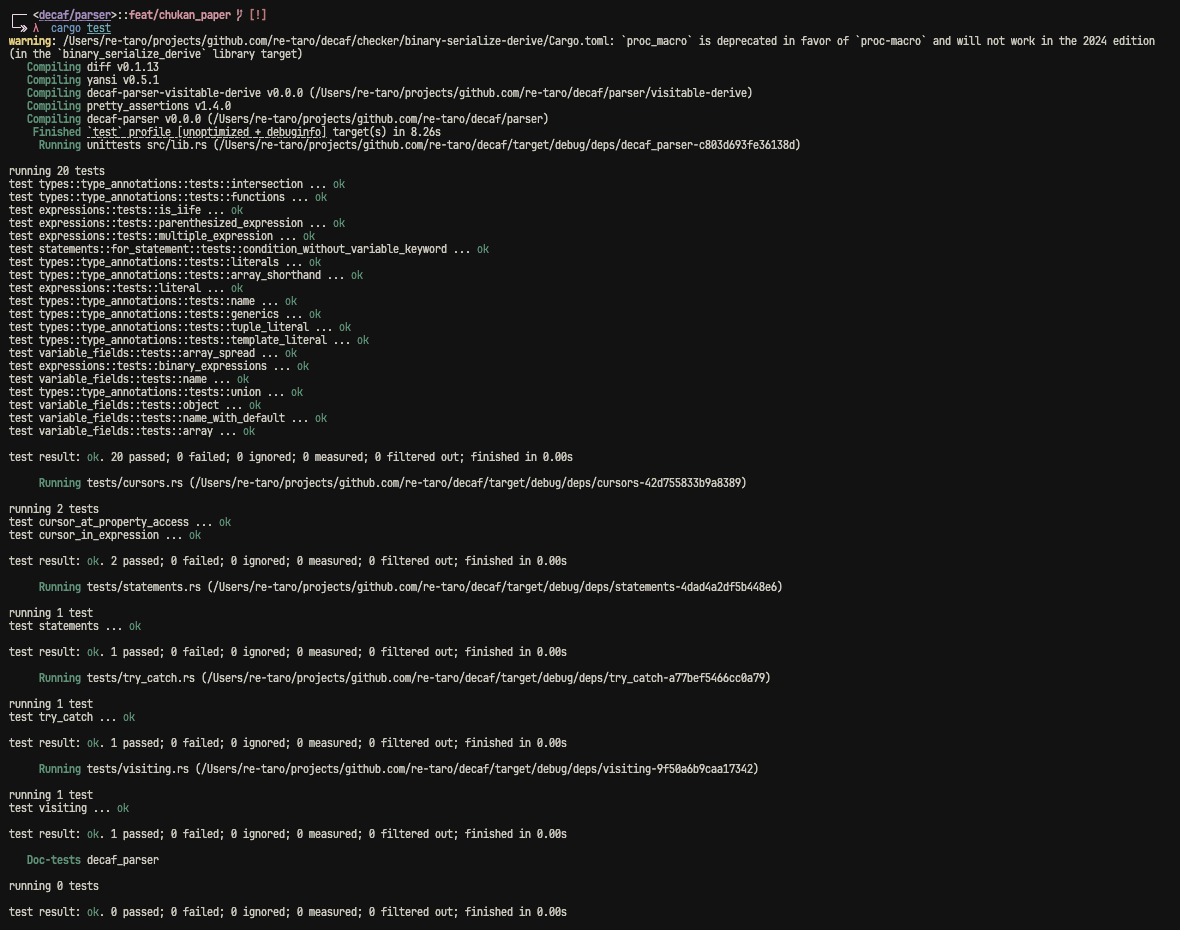
\includegraphics[width=0.85\columnwidth]{figures/parser_unit.png}
      \caption{パーサーのテスト結果}
      \label{fig:a}
  \end{minipage}
  \begin{minipage}[b]{0.49\columnwidth}
      \centering
      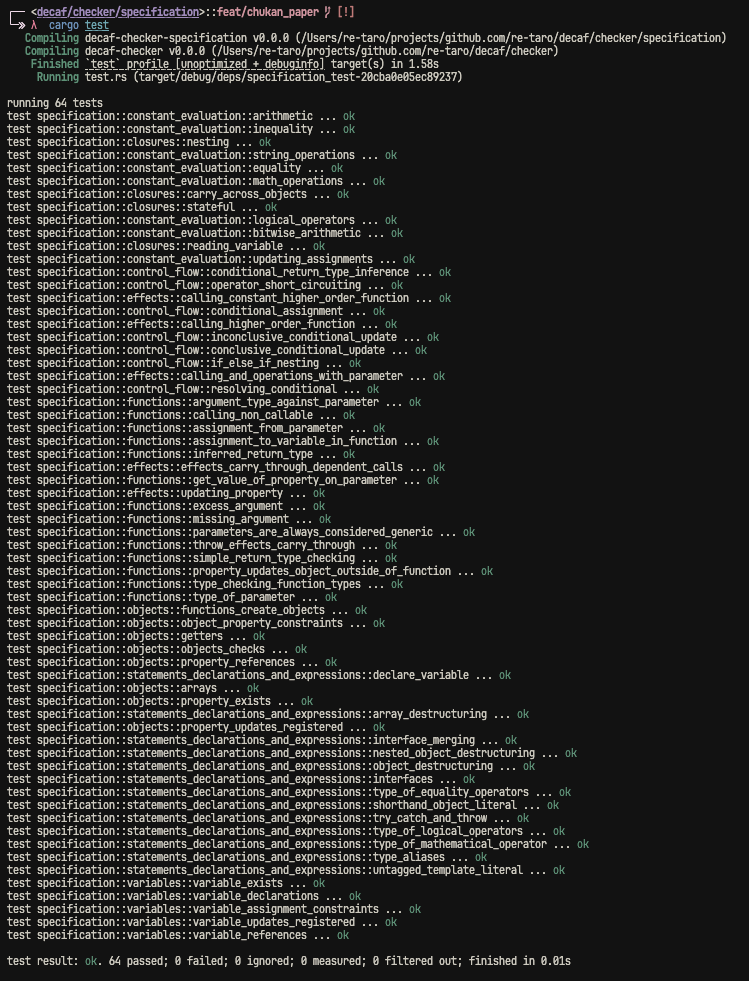
\includegraphics[width=0.85\columnwidth]{figures/chekcer_unit.png}
      \caption{型推論機のテスト結果}
      \label{fig:b}
  \end{minipage}
\end{figure}

\paragraph{<今後の方針>}
サポートする構文を増やし,型推論の精度を向上させる.
また,プレイグラウンドを作成し,フィードバックを受けやすい環境を整える.

\end{document}
